\begin{document}




\section{Komplettering}



\subsection{Jämviktsläget}

I vår rapport så tar vi upp jämviktsläget ganska kort när vi förklarar de krafter som påverkar systemet och hur vi räknar på utsignalen. Vi fick kommentaren att jämviktsläget är otydligt från figuren. Vi gjorde en ny bild som förklarar jämvikten så är krafterna och jämvikten förklarade separat.

\begin{figure}[h]
\begin{center}
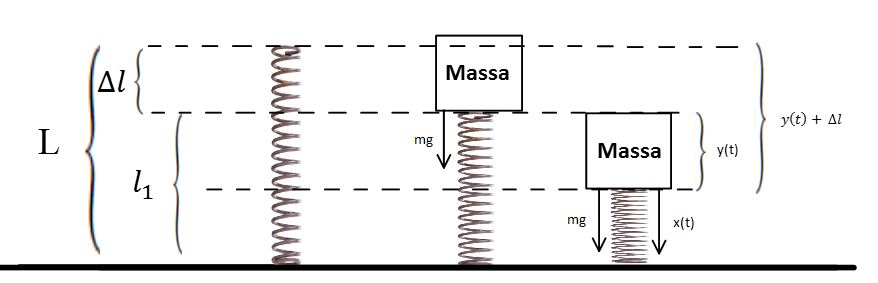
\includegraphics[scale=0.6]{jamvikt}
\caption{Förtydligande av jämnvikt}
\end{center}
\end{figure}

Fjädern utan en massa har jämviktsläget vid längd $L$. När man lägger på massan får den ett nytt jämviktsläge som vi kallar för $l_1$. Skillnaden mellan $L$ och $l_1$ är $\Delta l$. Sedan definierar vi en kraft $x(t)$ som verkar utöver gravitationen och skillnaden mellan det nya läget och $l_1$ som $y(t)$. Då blir den totala skillnaden $y(t) + \Delta l$

\subsection{Dämpningskraft}

Vi glömde i den ursprungliga rapporten att både visualisera dämpningskraften och nämna den i text. I den uppdaterade figuren nedan visas hur dämpningskraften ser ut i vårt fall med studsmattan, samt andra krafter som medverkar i systemet. Således betecknar vi dämpningskraften $F_d$, som är den kraft som motverkar rörelsen i ett svängningssystem motriktat rörelsen.

\begin{figure}[ht]
\begin{center}
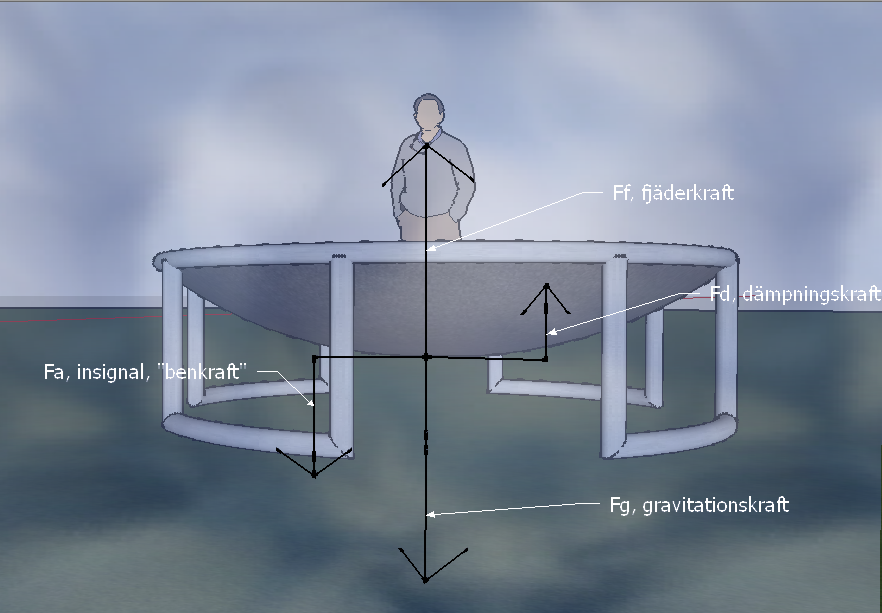
\includegraphics[scale=0.7]{shysstapilar}
\caption{Utsträckning för en fjäder}
\end{center}
\end{figure}
\newpage
\subsection{Differentialekvationen}

Med de verkande krafterna i systemet $F_a = x(t), F_g = mg, F_f = -k(\Delta l + y(t),F_d = -cv$ och med Newtons andra lag fick vi fram ekvationen:
\begin{equation}
F_tot = x(t) + mg - k(\Delta l + y(t)) - cv = ma
\end{equation} 
Där $x(t)$ är insignalen, $y(t)$ är utsignalen, $k$ är fjäderkonstanten, $c$ är dämpningskonstanten, $m$ är personen på mattans massa, $v$ är hastigheten, $a$ är accelerationen och $g$ är gravitationen. Om vi då uttrycker acceleration och hastighet som funktioner av tiden så kan vi uttrycka en differentialekvation.
\begin{equation}
a = \frac{d^2y(t)}{dt^2} , v = \frac{y(t)}{dt}
\end{equation}
Vilket ger:
\begin{equation}
 m\frac{d^2y(t)}{dt^2} =  -k(\Delta l + y(t)) -c\frac{dy(t)}{dt} + mg +  x(t)
\end{equation}

I det sista steget för den slutgiltiga differentialekvationen så fick vi kommentaren att vi skulle visa ett steg mer matematiskt. Vi skrev kort och gott att vid tid $t = 0$ så kommer gravitationen och fjäderkraften som verkar på massan ta ut varandra, och därav befinna sig i jämvikt.

För att detta ska vara tillräckligt bör vi visa hur detta kommer sig. Vi kan visa detta genom att utgå från ekvation ((X)).
\begin{equation}
\begin{split}
 m\frac{d^2y(t)}{dt^2} =  -k(\Delta l + y(t)) -c\frac{dy(t)}{dt} + mg +  x(t) \\ \leftrightarrow m\frac{d^2y(t)}{dt^2} = x(t) + mg  - k \Delta l -  k y(t)) -c\frac{dy(t)}{dt}  
\end{split}
\end{equation}
Om vid $t = 0$ både insignal $x(0) = 0$ och utsignal $y(0) = 0$ så får vi bara kvar
\begin{equation}
0 = mg  - k \Delta l
\end{equation}
Om vi stoppar in detta samband i ekvation ((X)) så får vi vår slutgiltiga differentialekvation:
\begin{equation}
\begin{split}
m\frac{d^2y(t)}{dt^2} = x(t) + mg  - k \Delta l -  k y(t)) -c\frac{dy(t)}{dt} \\ \leftrightarrow
 m\frac{d^2y(t)}{dt^2} + k  y(t) + c\frac{dy(t)}{dt} = x(t)
 \end{split}
\end{equation}

\subsection{Val av konstanter}

I rapporten så använde vi oss av ett par konstanter för att vi skulle kunna räkna och testa vår modell av systemet. Vi fick dock kommentaren att vi borde motivera dem. Vi hade inte valt dem helt slumpmässigt, men vår motivation var uppenbarligen inte med.

Massan är den vi utgick från. Vi valde $m = 70$ eftersom det är en vanlig vikt på en normalstor person. För att ta fram fjädringskonstanten funderade vi över hur djupt i mattan personen skulle sjunka (dvs, hur mycket fjädern skulle tryckas ihop). Vi valde $k = 2000$, för då skulle det krävas 1000 N för att sjunka ned/trycka ihop 0.5 m, varpå vår person skulle sjunka 0.35 m. Detta är ganska rimligt. Dämpningskonstanten är dock mer eller mindre omöjlig för oss att kontrollera. Vi ville dock med studsmattan skapa en så hög amplitud som möjligt, med mycket svängning och lite dämpning. Detta återfinns i det fallet då systemfunktionen har två komplexa rötter. Då fick vi ett krav på dämpningskonstanten för att det skulle vara ett sådant system. Kravet var
\begin{equation}
(\frac{c}{2m})^2 - \frac{k}{m} < 0
\end{equation}
Givet detta med de konstanter vi redan hade så valde vi $c = 100$.

\subsection{Laplacetransform}
Vi fick i vår ursprungliga rapport knappt med någon förklaring om varför vi tillämpar laplacemetoden i vår systemundersökning. En laplacetransformerad funktion är ett användbart verktyg för att undersöka ett systems egenskaper. Transformationen avbildar en funktion i tidsdomänen, på en annan funktion i frekvensdomänen. Laplacetransformen är särskilt användbar då man undersöker system som inte är energifria, vilket andra metoder för systemanalys, så som fouriertransformering och faltning, inte kan hantera. I vårt fall med studsmattan är systemet emellertid energifritt, men laplacetransformationen kan i detta fall ändå tillämpas och ger dessutom lättare algebraiska manipulationer än alternativa metoder.
Efter laplacetransformering av systemets signalförhållande kan systemets så kallade systemfunktion utvinnas, vilket kan användas för analysera systemet ytterligare.

När man laplacetransformerar så finns det färdiga standardtransformer man kan utgå ifrån för att slippa långa och invecklade integralberäkningar. Dessa finns i t.ex. formelsamlingen "Formler och tabeller" av Sune Söderkvist. Vi fick frågan vaför vi använde en specifik tabell när vi tog fram impulssvaret, och det var ju då just för att vi hade en systemfunktion som var på samma form som laplacetransformen i tabell 19.23 i den formelsamlingen.

\subsection{Stabilitetsbevis}

Vi gjorde ett väldigt långt stabilitetsbevis och försökte vara väldigt noggranna, men vi borde ha tagit med det enkla stabilitetsbeviset också. Vi fick nämligen kommentaren att det var väldigt omständigt och skulle lösas på annat sätt. Dessutom fick vi frågan "Vad är stabilitet?"

Stabilitet med avseende på ett fysikaliskt system innebär att varje begränsad insignal ger en begränsad utsignal. Ett sätt att bevisa stabilitet hos ett system är att visa att frekvensfunktionen $H(\omega)$ existerar. Vi har systemfunktionen $H(S)$ och kan därav dels kolla på noll-pol diagrammet om den imaginära axeln ($j\omega$-axeln) är med i konvergensområdet, och dels se efter om antalet poler är lika med eller fler än antalet nollställen. Om både dessa krav är uppfyllda hade det visat att systemet är stabilt. 

Systemet är kausalt då dess utsignal enbart beror på nu- och dåtida insignaler. Vi har även visat att systemet är linjärt och tidsinvariant i rapporten. Därav följer att eftersom systemet är ett kausalt LTI system så kommer konvergensområdet ligga till höger om polerna enligt bild ((X)). Vi ser även att antalet poler är fler än antalet nollställen, dvs. inga. Därmed är de två kraven uppfyllda, vilket visar att systemet är stabilt.

\begin{figure}[h]
\begin{center}
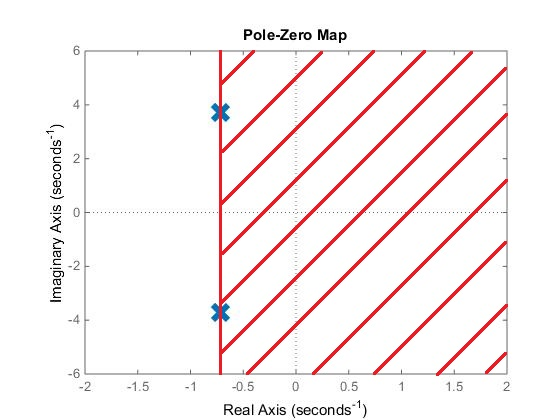
\includegraphics[scale=0.6]{nolpol-diagram_konvergens}
\caption{Pol-nollställediagram med konvergensområde}
\end{center}
\end{figure}

Detta visar dessutom hur vi går från vår systemfunktion till frekvensfunktionen i rapporten som också behövde motiveras. Detta behövde motiveras eftersom vi inte använde detta stabilitetsbevis i rapporten och därav blev förklaringen kring detta väldigt kortfattad. 

Men med detta stabilitetsbevis så är det väldigt nära att då visa att $j\omega$ är med i konvergensområdet och vi kan då säga att $s = \sigma + j\omega$. Då $\sigma = 0$ så har vi frekvensfunktionen $H(s) = H(\omega), s = j\omega$

\subsection{Stegsvar}

I vår rapport så tog vi fram stegsvaret, $g(t)$, genom att integrera impulssvaret, $h(t)$. Vi fick kommentaren att det går att lösa på ett enklare sätt. 

En enklare metod för att ta fram g(t) är att utnyttja sambandet $Y(s) = X(s)H(s)$ så att $G(s) = U(s)H(s)$. Därefter får vi stegsvaret $g(t)$ genom att inverslaplacetransformera $G(s)$.

Vi laplacetransformerar först enhetssteget $\mathcal{L}(u(t)) = \frac{1}{s} = U(s)$ och multiplicerar detta med systemfunktionen $H(s)$
\begin{equation}
U(s)H(s) = \frac{1}{s} \frac{1}{ms^2 + cs + k}
\end{equation}
Genom att uttrycka systemfunktionen $H(s)$ med dess rötter istället blir det enklare att räkna med. Rötterna i vårt fall med studsmattan har redan beräknats konkret i rapporten. Vi betecknar därmed rötterna som $r_1, r_2$ och får då 
\begin{equation}
\frac{1}{m} \frac{1}{(s - r_1) (s - r_2)}
\end{equation}
För att enkelt kunna inverslaplacetransformera uttrycket partialbråksupdelar vi uttrycket och får då:

\begin{equation}
\frac{1}{m} \left(\frac{A}{s} + \frac{B}{s - r_1} + \frac{C}{s - r_2}\right)
\end{equation}

Vi beräknar A, B, C och inverslaplacetransformerar uttrycket så får vi:
\begin{equation}
\mathcal{L}^-1\left\lbrace \frac{1}{m} \left( \frac{1}{s(r_1 r_2)} - \frac{1}{r_1(s-r_1)(r_2-r_1)} + \frac{1}{r_2(s-r_2)(r_2 - r_1}   \right) \right\rbrace
\end{equation}
Och detta ger oss stegsvaret $g(t)$

\begin{equation}
g(t) = \frac{1}{m} \left( \frac{1}{r_1 r_2} - \frac{1}{\frac{r_1}{r_2} - r_1} e^{r_1t} + \frac{1}{r_2(r_2 - r_1)} e^{r_2 t}   \right) u(t)
\end{equation}


\subsection{Amplitud- och faskaraktäristik}

Vi gav en lite klumpig beskrivning av vad amplitud- och faskaraktäristik är för något och fick kommentaren att vi måste förtydliga detta.

Vi skrev att amplitud- och faskaraktäristiken beskriver hur impulssvarets amplitud och fasförskjutning påverkas av insignalens frekvens. Det är inte riktigt korrekt. Det är sant att den påverkas, men det är inte bara impulssvaret som påverkas eftersom den endast uppkommer om insignalen är en dirac. Alla utsignaler kommer se olika ut beroende på vilken frekvens insignalen har.

\subsection{Impuls- och stegsvar för olika system}

Om man varierar de olika konstanterna så får man olika system med olika egenskaper. Vi gjorde några sådana tester med fas- och amplitudkaraktäristik, men inte med impuls- eller stegsvaret. Impulssvaret och stegsvaret är centrala i ett systems beteende och vi borde ha diskuterat dessa. Här följer både impulssvar och stegsvar med variation av konstanterna.

\begin{figure}[h]
\begin{center}
\includegraphics[scale=0.4]{impulssvar(massa)}
\caption{Impulssvar med varierande massa}
\end{center}
\end{figure}

I figur 27 kan man se att massan ger lite skillnad i både amplitud och frekvens. Eftersom kraften är densamma så kommer den lätta massan få högre amplitud eftersom gravitationen påverkar mindre. Man kan också se att den tunga personen svänger under en längre period på grund av rörelsemängden.

\newpage
\begin{figure}[h]
\begin{center}
\includegraphics[scale=0.4]{impulssvar(fjader)}
\caption{Impulssvar med varierande fjäderkonstant}
\end{center}
\end{figure}

Figur 28 visar att med en väldigt hög fjäderkonstant så får systemet en väldigt liten amplitud och hög frekvens. Detta för att fjädern är så stark att den trycker tillbaka med stor kraft väldigt snabbt. Med den låga fjäderkonstanten har man istället en mycket hög amplitud och låg frekvens. Det första man kan konstatera är att den förmodligen slår i backen för att studsmattan inte är så hög. Detta beteende kommer ifrån att fjädern inte är så stark så det krävs en lång amplitud för att den ska ta ut insignalen. 

\begin{figure}[h]
\begin{center}
\includegraphics[scale=0.4]{impulssvar(dampning)}
\caption{Impulssvar med varierande dämpningskonstant}
\end{center}
\end{figure}

I figur 29 nedan ser vi att med låg dämpning så kommer systemet svänga väldigt länge. Då finns det knappt någon kraft som ständigt jobbar emot svängningen, vilket ger en väldigt långvarig svängning. Motsatsen blir ju då självklart att den inte svänger alls på grund av den starka kraften som ständigt jobbar emot svängningen.
\newpage

\begin{figure}[h]
\begin{center}
\includegraphics[scale=0.4]{stegsvar(massa)}
\caption{Stegsvar med varierande massa}
\end{center}
\end{figure}

Figur 30 visar att för en högre massa så tar det längre tid att svänga in till det nya jämnvikts läget, detta av samma anledning som vid impulssvaret. Hur mycket det skilljer sig från jämnviktsläget är inte beroende på massan då olika massor ger olika startjämnviktslägen

\begin{figure}[h]
\begin{center}
\includegraphics[scale=0.4]{stegsvar(fjader)}
\caption{Stegsvar med varierande fjäderkonstant}
\end{center}
\end{figure}

Figur 31 visar att fjäderkonstanten har stor påverkan på det nya jämnviktsläget. Med en hög fjäderkonstant så förändras inte jämnviktsläget så mycket efter som det krävs stor kraft för att dra ut fjädern. Det motsatta gäller för låga fjäderkonstanter.

\begin{figure}[h]
\begin{center}
\includegraphics[scale=0.4]{stegsvar(dampning)}
\caption{Stegsvar med varierande dämpningskonstant}
\end{center}
\end{figure}

I figur 32 ser vi att dämpningskonstaten är vital i hur systemet fungerar. Vid en för hög dämpningskonstant får vi ingen studseffekt utan man sjunker sakta men säkert in i det nya jämnviktsläget. För et för låg dämpningskonstant så oscillerar man runt jämnviktsläget orimligt länge.
\end{document}